% Delegation decision — funnel: each "no" exits to "Do it directly"; pass all
% three and "Delegate". Pedagogy pass: terse labels, neutral decision diamonds,
% color reserved for the outcome (Delegate=green). Warm-Tol brand hues.
\documentclass[tikz,border=4mm]{standalone}
\usepackage{tikz}
\usetikzlibrary{positioning, shapes.geometric, arrows.meta, calc}

\definecolor{warmgreen}{HTML}{4A7E3F}

\begin{document}
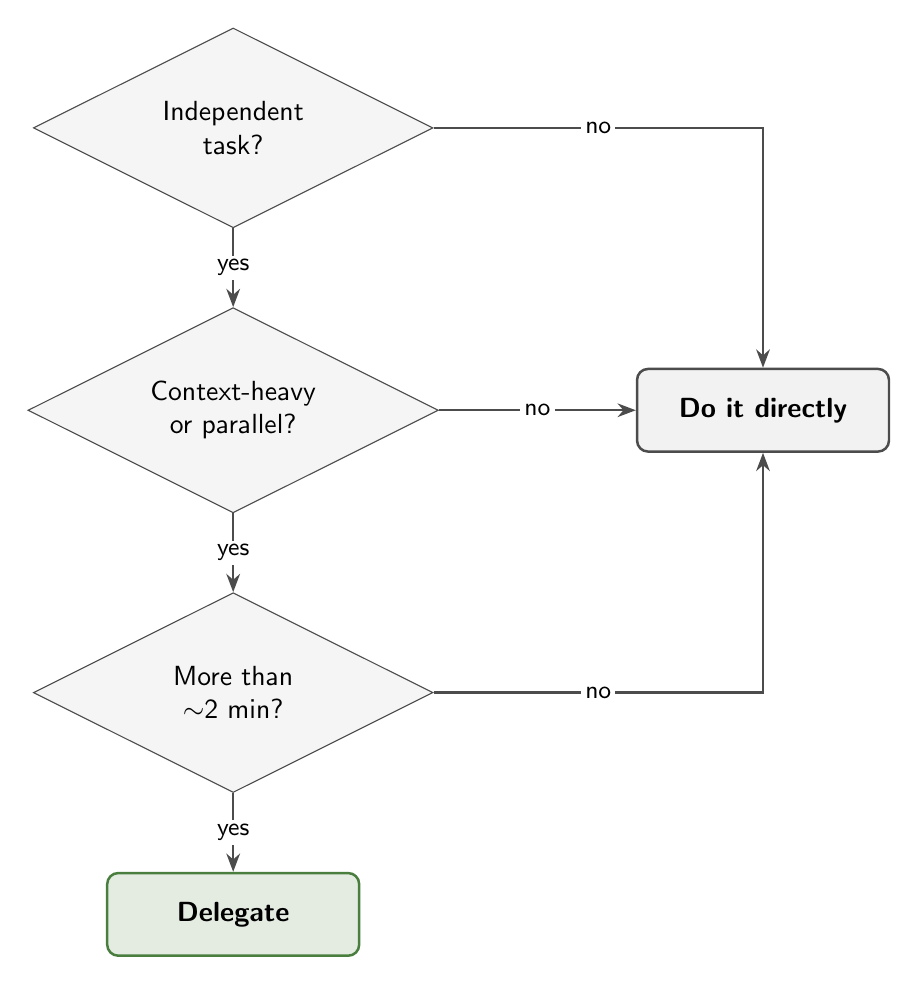
\begin{tikzpicture}[
  font=\sffamily,
  node distance=1.0cm and 2.5cm,
  question/.style={
    draw=gray!60!black, fill=gray!8, diamond, aspect=2.0,
    inner sep=4pt, align=center, text width=2.9cm, font=\sffamily
  },
  ep/.style={
    rounded corners=4pt, minimum width=3.2cm, minimum height=1.05cm,
    inner sep=6pt, align=center, font=\sffamily\bfseries, line width=0.9pt
  },
  epgreen/.style={ep, draw=warmgreen, fill=warmgreen!15},
  epneutral/.style={ep, draw=gray!60!black, fill=gray!10},
  arrow/.style={-Stealth, thick, draw=gray!60!black},
  arrowlabel/.style={font=\sffamily\small, fill=white, inner sep=1.5pt},
]

\node[question] (q1) {Independent \\ task?};
\node[question, below=of q1] (q2) {Context-heavy \\ or parallel?};
\node[question, below=of q2] (q3) {More than \\ $\sim$2 min?};
\node[epgreen, below=of q3] (del) {Delegate};

\node[epneutral, right=of q2] (direct) {Do it directly};

\draw[arrow] (q1) -- node[arrowlabel] {yes} (q2);
\draw[arrow] (q2) -- node[arrowlabel] {yes} (q3);
\draw[arrow] (q3) -- node[arrowlabel] {yes} (del);

\draw[arrow] (q1.east) -| node[arrowlabel, near start] {no} (direct.north);
\draw[arrow] (q2.east) -- node[arrowlabel] {no} (direct.west);
\draw[arrow] (q3.east) -| node[arrowlabel, near start] {no} (direct.south);

\end{tikzpicture}
\end{document}
